\documentclass[slides]{pgnotes}

\title{Ansible}

\begin{document}

\maketitle

\tableofcontents

\section{Scenario}

\begin{center}
  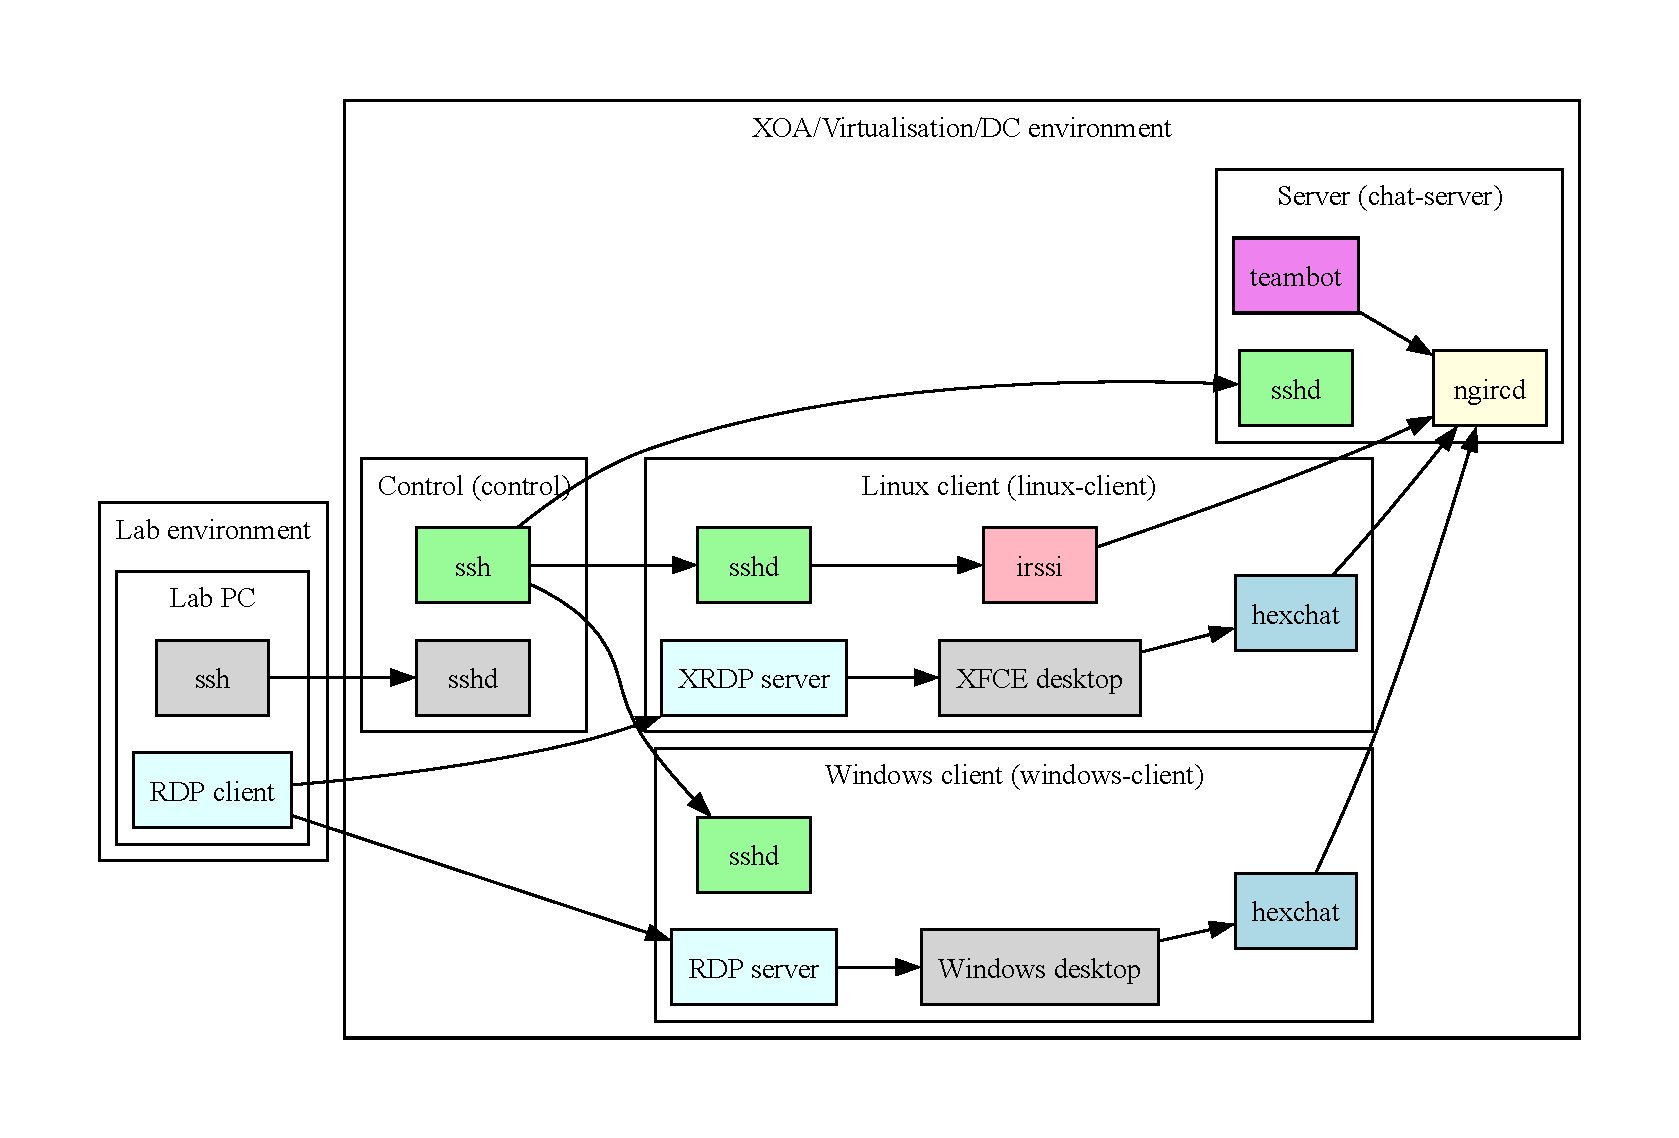
\includegraphics[width=1.0\linewidth]{scenario}
\end{center}


\subsection{Components}

\begin{description}
\item[Control node]: System where we will be automating things frmo.
  \begin{itemize}
  \item So far you could issue SSH commands from here.
  \item Today we will run Ansible commands such as \texttt{ansible} or \texttt{ansible-inventory} on the control node.
  \end{itemize}
  
\item[Managed node]: Remote system, or host, that we want to control.
  \begin{itemize}
  \item Commands etc will be run here remotely over SSH.
  \item May be physical, virtual, cloud VM, SBC like R-Pi etc.
  \item Commands will be issued today by Ansible system.
  \end{itemize}

\item[Inventory]: List of managed nodes that are logically organized.
  \begin{itemize}
  \item Can create inventory on the control node to describe host deployments to Ansible.
  \end{itemize}

  
\end{description}

\subsection{Set-up}

\textbf{To save lab time, let's start the set up the 3 machines now (Task 1)!}


\subsection{Common automation tasks}

\begin{enumerate}
\item Package update
\item Software installation
\item Service configuration (enabled / disabled)
\item Local user account management (creation, deletion)
\item Local group management (creation, deletion, membership)
\item Configuration file maintenance
\end{enumerate}

\section{Ansible}

Ansible is an open-source automation solution that reduces complexity and runs on a variety of operating systems.

\begin{greenbox}{Common use cases for Ansible}
\begin{itemize}
\item Eliminate repetition and simplify workflows
\item Manage and maintain system configuration
\item Continuously deploy complex software
\item Perform zero-downtime rolling updates
\end{itemize}
\end{greenbox}


\subsection{Design principles}

\begin{enumerate}
\item \textbf{Agent-less architecture:}
Low maintenance overhead by avoiding the installation of additional software across IT infrastructure.

\item \textbf{Simplicity:}
  Automation playbooks use straightforward YAML syntax for code that reads like documentation. Ansible is also decentralized, using SSH with existing OS credentials to access to remote machines.

\item \textbf{Scalability and flexibility:}
Easily and quickly scale the systems you automate through a modular design that supports a large range of operating systems, cloud platforms, and network devices.

\item \textbf{Idempotence and predictability:}
When the system is in the state your playbook describes Ansible does not change anything, even if the playbook runs multiple times.
\end{enumerate}


\subsection{Agentless architecture}

Ansible is \textbf{agentless}:
\begin{itemize}
\item Some automation solutions require an \textit{agent} to be running on the managed node(s).
\item Ansible uses SSH to let the control node take actions on the managed node.
\item Once you can make an SSH connection from the control to the mangaged node you can run ansible commands on it.
\end{itemize}

\begin{redbox}{Pre-requisitites}
  The agentless architecture practically requires the following:
  \begin{enumerate}
  \item We can make an SSH connection from the control to the managed node.
  \item The SSH connection can happen without a password (i.e. with keys)
  \item The user we connect as can run commands as root without a password
  \item The target host is powered on and connected. (Consider Ansible Pull for Desktops)
  \end{enumerate}
\end{redbox}

\section{Inventory}

\textbf{Hosts} managed by ansible are listed in the \textit{inventory}:

\begin{itemize}
\item Simplest inventory is a text file.
  \begin{itemize}
  \item Default location \texttt{/etc/ansible/hosts}
  \item Can put elsewhere using the \texttt{-i} flag
  \end{itemize}
\item Can integrate ansible with other data sources to supply inventory
  \begin{itemize}
  \item Can even write your own in code
  \end{itemize}
\end{itemize}

\textbf{Groups} allow us to select multiple hosts at the same time.


\subsection{Inventory file example}

\inputminted{ini}{inventory_example.ini}


\section{Playbooks}

Ansible automation tasks are defined in \textbf{Playbooks}, in YAML format:

\begin{description}
\item[Playbook:] text file containing multiple \textit{plays}
\item[Play:] executes part of the overall goal of the playbook, running one or more \textit{tasks}.
\item[Task:] Each task calls an Ansible \textbf{module}
\end{description}

Ansible modules are prepackaged functionality in Ansible that avoids us having to script simple operations (e.g. package installation)

\begin{bluebox}{Each play must define}
  \begin{enumerate}
  \item The managed \textbf{nodes} to target
  \item At least one \textbf{task} to execute
  \end{enumerate}
\end{bluebox}


\subsection{Idempotency}

Most Ansible modules
\begin{enumerate}
\item Check whether the desired final state has already been achieved, and
\item Exit without performing any actions if that state has been achieved,
  \begin{itemize}
    \item So that repeating the task does not change the final state.
  \end{itemize}
\end{enumerate}

Modules that behave this way are often called ``idempotent'':
\begin{itemize}
\item Whether you run a playbook once, or multiple times, the outcome should be the same.
\item However, not all playbooks and not all modules behave this way.
\end{itemize}


\end{document}

